\secnumbersection{PROPUESTA DE SOLUCIÓN}

% Se debe desarrollar la solución propuesta. Los subcapítulos por poner aquí son propios del autor. Se sugiere mencionar metodología usada. Es conveniente incorporar figuras y tablas para aclarar la solución, que deben indicar el número de la figura, su nombre y su autor o fuente (si las diseñas tú, la fuente es ``Elaboración propia''). Ver ejemplos en esta página y en la siguiente.

% Cabe mencionar que aquí está la esencia del trabajo en lo que se refiere al aporte creativo del memorista, es el momento de demostrar que usted es un destacado profesional que creó, diseñó y/o llevó a cabo la solución propuesta.

Esta propuesta presenta la evolución de \textbf{DRAFTS} \cite{zhang2024drafts} desde un prototipo de investigación hacia un \textit{pipeline} \textbf{productivo, robusto y eficiente} diseñado para operaciones observacionales a gran escala. La transformación arquitectónica no se limita a mejoras incrementales, sino que establece una \textbf{extensión fundamental para regímenes de alta frecuencia} que expande significativamente las capacidades de detección en el espectro milimétrico.

\subsection{Vista General: Dos Grandes Bloques de Contribución}

Esta propuesta se estructura en \textbf{dos grandes bloques} que abordan desafíos complementarios en la detección de FRBs:

\textbf{Bloque 1: DRAFTS++ - Pipeline Productivo, Robusto y Eficiente} aborda la transformación del prototipo DRAFTS original hacia un sistema productivo capaz de operar en entornos observacionales reales. Este bloque incluye la refactorización arquitectónica completa, implementación de procesamiento eficiente por chunks, trazabilidad completa y artefactos de salida estandarizados.

\textbf{Bloque 2: Extensión a Alta Frecuencia - Cuatro Líneas de Investigación} explora estrategias metodológicas para extender las capacidades de detección hacia regímenes de alta frecuencia (30-100 GHz), donde las firmas dispersivas tradicionales se atenúan significativamente. Este bloque presenta cuatro líneas de investigación complementarias que abordan diferentes aspectos del desafío de detección en el espectro milimétrico.

\subsection{Bloque 1: DRAFTS++ - Pipeline Productivo, Robusto y Eficiente}

Este bloque aborda la transformación fundamental del prototipo DRAFTS original hacia un sistema productivo capaz de operar en entornos observacionales reales. La evolución desde un prototipo de investigación hacia sistema productivo requiere una transformación arquitectónica fundamental que aborde las limitaciones inherentes del código base original.

\subsubsection{Desafíos del Prototipo Original}

El prototipo inicial presenta una estructura monolítica con scripts independientes (\texttt{d-center-main.py}, \texttt{d-resnet-main.py}) optimizados para condiciones de laboratorio controladas pero incapaces de manejar la variabilidad operacional de entornos observacionales reales. Las limitaciones principales incluyen:

\begin{itemize}
\item \textbf{Estructura monolítica:} Scripts independientes sin integración coherente
\item \textbf{Procesamiento limitado:} Lectura monolítica de archivos grandes sin gestión de memoria
\item \textbf{Falta de trazabilidad:} Ausencia de logging estructurado y reproducibilidad
\item \textbf{Salidas inconsistentes:} Figuras y reportes ad hoc sin estandarización
\item \textbf{Escalabilidad limitada:} Sin soporte para procesamiento distribuido o streaming
\end{itemize}

\subsubsection{Arquitectura Modular y CLI Unificada}

\noindent\textbf{Refactorización arquitectónica sistemática.} La transformación implementa una arquitectura modular con 11 componentes especializados que establecen separación clara de responsabilidades y interfaces estandarizadas. Esta reestructuración elimina las dependencias circulares del prototipo original y establece un flujo de datos unidireccional que garantiza consistencia operacional y facilita mantenimiento y extensibilidad del sistema.

Los módulos especializados incluyen:
\begin{itemize}
\item \textbf{I/O:} Manejo unificado de formatos FITS/PSRFITS/Filterbank
\item \textbf{Preprocesamiento:} Normalización, RFI mitigation y preparación de datos
\item \textbf{Propuesta de candidatos:} Estrategias intercambiables de detección
\item \textbf{Clasificación:} Redes neuronales para validación binaria
\item \textbf{Validador:} Verificación DM-aware y consistencia temporal
\item \textbf{Visualización:} Generación automática de plots y reportes
\end{itemize}

Se implementa una \textit{CLI} unificada con archivos de configuración validados (YAML/JSON) que permiten control granular de todos los parámetros del pipeline. Se fijan semillas, versiones y \textit{hashes} de datos/modelos para garantizar trazabilidad completa.

\subsubsection{Ingesta y Streaming por Chunks}

El sistema procesa archivos FITS/PSRFITS mediante algoritmos de normalización por canal que compensan variaciones instrumentales y efectos de ganancia. Se implementa enmascarado adaptativo de interferencia de radiofrecuencia (RFI) basado en análisis estadístico de outliers temporales y espectrales. 

La arquitectura de \emph{chunking} con solapamiento controlado permite procesamiento eficiente de observaciones de larga duración mediante streaming de datos con gestión automática de memoria. Esta aproximación elimina las limitaciones de memoria del prototipo original y permite procesar observaciones de cualquier duración.

\begin{figure}[H]
\centering
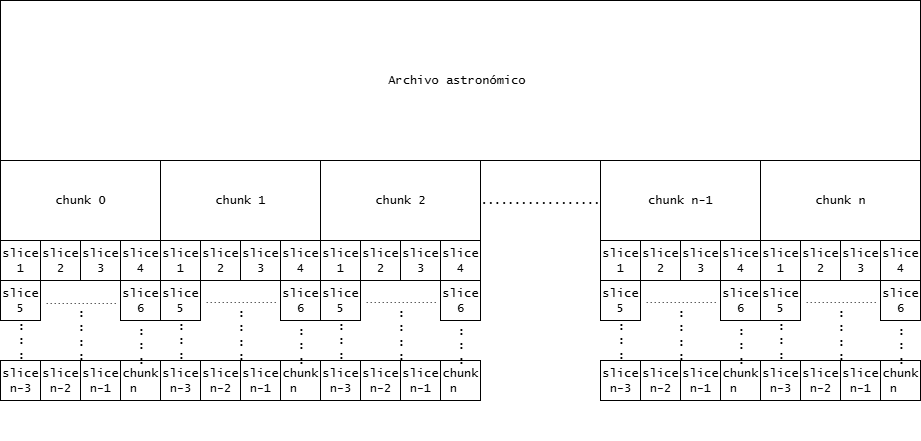
\includegraphics[width=0.9\textwidth]{figures/sistema-chunks.png}
\caption{Esquema de un archivo astronómico dividido en chunks y slices, ilustrando el concepto de procesamiento con solapamiento. Fuente: Elaboración propia.}
\label{fig:sistema-chunks}
\end{figure}

\subsubsection{Aceleración y Control de Recursos}

Vectorización de operaciones matemáticas críticas, integración opcional de procesamiento GPU para algoritmos intensivos en cómputo, y paralelización de bloques de procesamiento para maximizar la utilización de recursos computacionales disponibles. Se implementan \textit{caches} por canal y reducción de I/O para optimizar el rendimiento.

\subsubsection{Registro, Auditoría y Salidas Estandarizadas}

Sistema de \emph{logging} estructurado que registra todas las operaciones críticas, implementación de semillas fijas para algoritmos estocásticos, generación de firmas criptográficas para datos y modelos, y producción de resúmenes de métricas por ejecución para garantizar auditoría completa.

Las salidas incluyen reportes CSV/Parquet estructurados, figuras consistentes (tiempo--DM, dispersado/dedispersado, parches) y \textit{composites} que facilitan el análisis posterior y la validación de resultados.

\begin{table}[H] 
\centering 
  \caption{\label{tab:mejoras} Resumen de mejoras de ingeniería (DRAFTS++). \textit{Fuente: Elaboración propia}.}
\begin{tabular}{p{0.28\textwidth} p{0.32\textwidth} p{0.32\textwidth}} 
\toprule 
    \textbf{Aspecto} & \textbf{Antes (prototipo)} & \textbf{Después (DRAFTS++)} \\
\midrule 
Estructura & Scripts sueltos & Módulos + CLI + configs validadas \\ 
    Archivos grandes & Lectura monolítica & \emph{Chunking} + \emph{overlap} + control de memoria \\
    Detección & Sólo DL (DM--Time) & \emph{Strategy} intercambiable (DM--Time/TWL/SNR) \\
Auditoría & Log mínimo & Log estructurado + semillas + hashes \\ 
    Salidas & Figuras ad hoc & CSV/Parquet + plots estándar + composites \\
\bottomrule 
\end{tabular} 
\end{table}

\subsection{Bloque 2: Extensión a Alta Frecuencia - Cuatro Líneas de Investigación}

Este bloque explora estrategias metodológicas para extender las capacidades de detección hacia regímenes de alta frecuencia (30-100 GHz), donde las firmas dispersivas tradicionales se atenúan significativamente. La detección de FRBs en el régimen milimétrico presenta desafíos fundamentales que requieren aproximaciones metodológicas diferenciadas.

A estas frecuencias, la dispersión temporal se atenúa significativamente debido a la dependencia cuadrática inversa con la frecuencia, resultando en firmas dispersivas que pueden ser indistinguibles del ruido instrumental en resoluciones temporales típicas. Este bloque presenta cuatro líneas de investigación complementarias que abordan diferentes aspectos del desafío de detección en el espectro milimétrico.

\subsubsection{Línea 1: Validación de DRAFTS++ Sin Modificaciones}

\paragraph{Objetivo y Metodología}

Esta línea de investigación busca validar si DRAFTS++ con su arquitectura original (CenterNet en mapas DM-tiempo) puede mantener eficiencia aceptable en regímenes de alta frecuencia. Aunque se anticipa una reducción en el rendimiento debido a la atenuación de las firmas dispersivas, esta validación establece la línea base para comparar las mejoras de las otras líneas.

\paragraph{Criterio Físico para Evaluación}

Se utiliza el retardo dispersivo esperado frente a la resolución temporal como criterio de evaluación:
\[
\Delta t_{\mathrm{ms}} = 4.148808 \times 10^{3}\ \mathrm{DM}\,(\nu_{\mathrm{low}}^{-2}-\nu_{\mathrm{high}}^{-2}) \, .
\]

Cuando $\Delta t_{\mathrm{ms}} < \alpha\, t_{\mathrm{samp}}$ (p.ej., $\alpha\!=\!1.5$), el \textit{bow-tie} no sería resoluble y se espera una degradación significativa del rendimiento.

\subsubsection{Línea 2: Detección por SNR + Clasificación Binaria}

\paragraph{Metodología Híbrida}

Esta línea implementa una aproximación híbrida que combina la detección tradicional por SNR (similar a pipelines clásicos como PRESTO \cite{ransom_presto}) con la red de clasificación binaria de DRAFTS++. El proceso sigue estos pasos:

\begin{enumerate}
\item \textbf{Perfil temporal:} $s(t)$ $\rightarrow$ normalización robusta (mediana/MAD) $\rightarrow$ \textbf{SNR}(t)
\item \textbf{Detección de picos:} Hallazgo de máximos locales $\ge T$ con separación mínima $\Delta t_{\min}$
\item \textbf{Generación de cajas:} Para cada pico $t_i$: generar \textbf{caja sintética} $[t_i-w,\, t_i+w]$
\item \textbf{Dedispersión local:} Construir parche tiempo--frecuencia y dedispersar en rejilla local de DM
\item \textbf{Clasificación binaria:} Usar la red de clasificación de DRAFTS++ para determinar BURST/NO BURST
\item \textbf{Validación DM-aware:} Exigir DM$^\ast\!>\!0$ con incertidumbre acotada
\end{enumerate}

\paragraph{Ventajas de la Aproximación Híbrida}

Esta línea mantiene la eficiencia computacional de la detección por SNR (O(N)) mientras aprovecha la precisión de la red de clasificación entrenada de DRAFTS++. La activación automática del modo HF cuando $\Delta t_{\mathrm{ms}} < \alpha\, t_{\mathrm{samp}}$ garantiza que se use la estrategia más apropiada según las condiciones físicas.

\begin{figure}[H] 
\centering 
% \includegraphics[width=0.9\textwidth]{hf_mode_snr_boxes.pdf} 
\caption{\label{fig:hf} Modo HF: del perfil SNR a cajas sintéticas, dedispersión local y clasificación binaria. Fuente: Elaboración propia.} 
\end{figure}

\paragraph{Pseudocódigo de Detección SNR}

\begin{algorithm}[H]
\caption{Detección SNR para Alta Frecuencia}
\begin{algorithmic}[1]
\Input{$s(t)$, umbral $T$, separación mínima $\Delta t_{min}$}
\Output{Lista de picos candidatos $\{t_i\}$}
\Function{DetectarPicosSNR}{$s$, $T$, $\Delta t_{min}$}
    \State $s_{norm} \leftarrow (s - median(s)) / MAD(s)$
    \State $picos \leftarrow maxima\_locales(s_{norm})$
    \State $candidatos \leftarrow [\ ]$
    \For{$t$ \textbf{in} $picos$}
        \If{$s_{norm}[t] \geq T$ \textbf{and} $dist\_minima(t, candidatos) \geq \Delta t_{min}$}
            \State $candidatos.append(t)$
        \EndIf
    \EndFor
    \State \textbf{return} $candidatos$
\EndFunction
\end{algorithmic}
\end{algorithm}

\subsubsection{Línea 3: Nuevos Plots Característicos - TWL-maps}

\paragraph{Concepto de TWL-maps}

En el régimen de alta frecuencia, donde las firmas dispersivas tradicionales se atenúan significativamente, los mapas tiempo--ancho--polarización lineal (TWL) proporcionan información diagnóstica complementaria que puede compensar la pérdida de evidencia dispersiva. Estos productos especializados aprovechan la información de polarización disponible en observaciones con datos de Stokes completos.

\paragraph{Análisis de Polarización Lineal}

Cuando se dispone de datos de Stokes $I,Q,U$ \cite{hamaker1996understanding}, se puede calcular la \textbf{polarización lineal} $L=\sqrt{Q^2+U^2}$, que cuantifica la intensidad de la componente polarizada de la señal electromagnética. Esta medida proporciona información adicional sobre la naturaleza física de las fuentes y puede revelar patrones que no son evidentes en el análisis de intensidad total únicamente.

\paragraph{Flujo de Detección Híbrida TWL}

El proceso de detección híbrida sigue una secuencia específica que garantiza robustez y eficiencia:

\begin{enumerate}
\item \textbf{Evaluación de disponibilidad TWL:} El sistema verifica si \texttt{TWL\_HYBRID\_DETECTION} está habilitado y si los datos de polarización (Stokes Q, U) están disponibles.
\item \textbf{Generación de mapa t-W:} Si la detección híbrida está activa, se genera el mapa tiempo-ancho de ocupación de banda mediante \texttt{generate\_twl\_map\_for\_window}.
\item \textbf{Conversión a tensor RGB:} El mapa 2D se convierte a un tensor RGB de 512×512 píxeles usando \texttt{twl\_occupancy\_to\_detection\_tensor} para compatibilidad con CenterNet.
\item \textbf{Detección con CenterNet:} El tensor se procesa con la red de detección para identificar candidatos potenciales.
\item \textbf{Evaluación de candidatos:} Si se encuentran candidatos, se procede a clasificación binaria; si no, se activa el fallback SNR.
\item \textbf{Fallback SNR:} En caso de fallo de la detección híbrida o si está deshabilitada, se ejecuta \texttt{compute\_snr\_profile} y \texttt{\_find\_snr\_peaks} para detección tradicional.
\item \textbf{Clasificación final:} Todos los candidatos (híbridos o SNR) pasan por \texttt{classify\_patch} para determinar si son BURST o NO BURST.
\item \textbf{Guardado de resultados:} Los candidatos válidos se almacenan con métricas completas y se generan visualizaciones correspondientes.
\end{enumerate}

\begin{figure}[H]
\centering
\begin{tikzpicture}[
    node distance=1.2cm and 1.5cm,
    box/.style={rectangle, draw, fill=blue!20, text width=2.2cm, text centered, minimum height=0.7cm, font=\small},
    decision/.style={diamond, draw, fill=yellow!20, text width=1.8cm, text centered, minimum height=0.7cm, font=\small},
    process/.style={rectangle, draw, fill=green!20, text width=2.2cm, text centered, minimum height=0.7cm, font=\small},
    arrow/.style={-Stealth, thick}
]

% Nodos principales
\node[box] (A) {Pipeline Alta Frecuencia};
\node[decision, below=of A] (B) {TWL Híbrido?};
\node[process, below left=of B] (C) {Generar Mapa t-W};
\node[process, below=of C] (D) {Convertir a Tensor RGB};
\node[process, below=of D] (E) {Red de Detección};
\node[decision, below=of E] (F) {Candidatos?};
\node[process, below left=of F] (G) {Clasificación Binaria};
\node[process, below right=of B] (H) {Fallback SNR};
\node[process, below=of H] (I) {Detección SNR Tradicional};
\node[process, below=of G] (J) {Guardar Candidatos};

% Conexiones
\draw[arrow] (A) -- (B);
\draw[arrow] (B) -- node[left] {Sí} (C);
\draw[arrow] (C) -- (D);
\draw[arrow] (D) -- (E);
\draw[arrow] (E) -- (F);
\draw[arrow] (F) -- node[left] {Sí} (G);
\draw[arrow] (B) -- node[right] {No} (H);
\draw[arrow] (H) -- (I);
\draw[arrow] (I) -- (F);
\draw[arrow] (G) -- (J);

\end{tikzpicture}
\caption{\label{fig:hf-pipeline} Flujo del Pipeline de Alta Frecuencia: detección híbrida TWL con fallback automático a SNR tradicional. El diagrama muestra la decisión que determina si usar detección híbrida (mapa t-W + CenterNet) o fallback a SNR tradicional. Fuente: Elaboración propia.}
\end{figure}

\begin{figure}[H] 
\centering 
% \includegraphics[width=0.9\textwidth]{twl_map.pdf} 
\caption{\label{fig:twl} Ejemplo de TWL-map (tiempo vs. ancho con intensidad de $L$). Fuente: Elaboración propia.} 
\end{figure}

\subsubsection{Línea 4: Estrategias Alternativas del Autor de DRAFTS}

\paragraph{DM-range Expand \& Step Coarse}

Esta línea explora estrategias sugeridas por Yong–Kun Zhang \cite{zhang2024drafts} para maximizar la visibilidad de firmas dispersivas residuales. La metodología incluye:

\begin{itemize}
\item \textbf{Expansión del rango/step de DM:} Ampliar el rango y el \textit{step} de DM hasta "abrir" el \textit{bow-tie}
\item \textbf{Verificación estadística:} Una vez detectado, exigir centro con DM$>0$ significativamente mayor que cero
\item \textbf{Detección de candidatos cerca de DM$\approx 0$:} Mediante algoritmos de detección de picos adaptativos seguida de validación rigurosa
\end{itemize}

\paragraph{Fishing en DM$\approx 0$ + Chequeos Estrictos}

\textit{Pescar} candidatos con clasificador o detector simple cerca de DM$\approx 0$; luego validar con DM$>0$, consistencia por sub-bandas y coherencia entre \emph{chunks}. Útil para eventos débiles sin \textit{bow-tie} claro.

\paragraph{Integración con el Pipeline}

Ambas tácticas se exponen como \textbf{estrategias} de propuesta de candidatos (alternativas a SNR/TWL/DM--Time) y se someten al \textbf{mismo} validador DM-aware, clasificación y visualización.

\begin{table}[H] 
\centering 
\caption{\label{tab:estrategias} Estrategias de propuesta de candidatos y criterios de uso. Fuente: Elaboración propia.} 
\begin{tabular}{p{0.24\textwidth} p{0.38\textwidth} p{0.30\textwidth}} 
\toprule 
\textbf{Estrategia} & \textbf{Cuándo usarla} & \textbf{Pros / Contras} \\ 
\midrule 
CenterNet en DM--Time & $\Delta t \gg t_{\rm samp}$ (bow-tie resoluble) & + Precisa en L/S-band; -- Pierde poder en mm-wave \\ 
TWL-Híbrido + CenterNet & Stokes disponibles en mm-wave & + Usa polarización/anchos; -- Coste extra de features \\ 
SNR-only + Clasificador & mm-wave sin bow-tie claro & + O(N), simple; -- Más FP sin validación DM-aware \\ 
DM$\approx 0$ fishing + validar DM$>0$ & Para "pescar" candidatos débiles & + Sensible; -- Requiere validaciones estrictas \\ 
\bottomrule 
\end{tabular} 
\end{table}

\begin{table}[H]
  \centering
  \caption{\label{tab:param_hf} Parámetros del modo HF (valores iniciales). \textit{Fuente: Elaboración propia}.}
  \begin{tabular}{p{0.35\textwidth} p{0.55\textwidth}}
    \toprule
    \textbf{Parámetro} & \textbf{Descripción} \\
    \midrule
    $T$ (umbral SNR) & 5--7; ajustar por FDR y condiciones de ruido \\
    $\Delta t_{\min}$ & Múltiplo del ancho de pulso esperado \\
    Rejilla DM local & Centrada en 0; pasos gruesos y posterior refinamiento \\
    Sub-bandas & 2--4 particiones para coherencia \\
    Criterio DM & Requerir DM$^\ast>0$ (con error acotado) \\
    \bottomrule
  \end{tabular}
\end{table}

\subsection{Arquitectura Unificada y Diagramas}

\subsubsection{Arquitectura Unificada (Strategy + Validator + Visualizer)}

Se adopta un patrón \textbf{Strategy} para la \textbf{propuesta de candidatos} (intercambiable: DM--Time/CenterNet, TWL-híbrido, SNR, DM-expand, fishing en DM$\approx0$), con un \textbf{validador DM-aware} común y un \textbf{visualizador desacoplado}. La función de proceso se unifica como \texttt{process\_slice(..., strategy)}.

\begin{figure}[H] 
\centering 
% \includegraphics[width=0.96\textwidth]{arquitectura_unificada.pdf} 
\caption{\label{fig:arquitectura-unificada} Arquitectura unificada: Strategy (propuesta de candidatos) + Validador DM-aware + Visualizador. \textit{Fuente: Elaboración propia}.} 
\end{figure}

\paragraph{Bucle Unificado (Pseudocódigo)}

\begin{algorithm}[H]
\caption{Pipeline Unificado con Strategy Pattern}
\begin{algorithmic}[1]
\Input{$config$, $obs\_params$, $data\_files$}
\Output{Candidatos validados y métricas}
\Function{RunPipeline}{$config$, $obs\_params$}
    \State $strategy \leftarrow select\_strategy(config, obs\_params)$
    \For{$chunk$ \textbf{in} $stream\_data(\ldots)$}
        \State $cands \leftarrow strategy.propose(chunk, meta)$
        \For{$c$ \textbf{in} $cands$}
            \State $patch \leftarrow extract\_patch\_and\_dedisperse(chunk, c, local\_dm\_grid)$
            \State $y \leftarrow classifier.predict(patch)$
            \If{$y.is\_burst$ \textbf{and} $dm\_validate(patch)$ \textbf{and} $subband\_consistency(patch)$}
                \State $save\_candidate(patch, y, metrics)$
            \EndIf
        \EndFor
    \EndFor
    \State $visualize\_and\_summarize(run\_id)$
\EndFunction
\end{algorithmic}
\end{algorithm}

\subsubsection{Diagrama End-to-End del Pipeline}

La Figura \ref{fig:pipeline-end-to-end} sintetiza el flujo desde \texttt{main.py} hasta los resultados, con ramas clásica (DM--Time/CenterNet) y de alta frecuencia (TWL-híbrido, SNR) y \textit{fallbacks}.

\begin{figure}[H]
\centering
\begin{tikzpicture}[
    node distance=1.0cm and 1.5cm,
    box/.style={rectangle, draw, fill=blue!20, text width=2.0cm, text centered, minimum height=0.6cm, font=\tiny},
    decision/.style={diamond, draw, fill=yellow!20, text width=1.6cm, text centered, minimum height=0.6cm, font=\tiny},
    process/.style={rectangle, draw, fill=green!20, text width=2.0cm, text centered, minimum height=0.6cm, font=\tiny},
    output/.style={rectangle, draw, fill=orange!20, text width=2.0cm, text centered, minimum height=0.6cm, font=\tiny},
    arrow/.style={-Stealth, thick}
]

% FLUJO SIMPLIFICADO
\node[box] (A) {main.py};
\node[box, below=of A] (B) {run\_pipeline};
\node[box, below=of B] (C) {Cargar Modelos};

% ENTRADA DE DATOS
\node[box, right=of B] (D) {find\_data\_files};
\node[decision, below=of D] (E) {Tipo Archivo?};
\node[box, below left=of E] (F) {fits\_handler};
\node[box, below right=of E] (G) {filterbank\_handler};

% PROCESAMIENTO
\node[box, below=of E] (H) {streaming\_orchestrator};
\node[box, below=of H] (I) {Procesar Chunk};
\node[decision, below=of I] (J) {Frecuencia ≥ 8GHz?};

% PIPELINES
\node[box, below left=of J] (K) {Pipeline Alta Frecuencia};
\node[box, below right=of J] (L) {Pipeline Clásico};

% DETECCIÓN
\node[decision, below=of K] (M) {TWL\_HYBRID?};
\node[box, below left=of M] (N) {TWL + CenterNet};
\node[box, below right=of M] (O) {SNR Tradicional};
\node[process, below=of L] (P) {CenterNet DM-Time};

% CLASIFICACIÓN
\node[process, below=of N] (Q) {classify\_patch};
\node[process, below=of O] (R) {classify\_patch};
\node[process, below=of P] (S) {classify\_patch};

% RESULTADOS
\node[output, below=of Q] (T) {Guardar Candidatos};
\node[output, below=of R] (U) {Guardar Candidatos};
\node[output, below=of S] (V) {Guardar Candidatos};

% VISUALIZACIÓN
\node[output, below=of T] (W) {Plots + CSV};
\node[output, below=of U] (X) {Plots + CSV};
\node[output, below=of V] (Y) {Plots + CSV};

% Conexiones principales
\draw[arrow] (A) -- (B);
\draw[arrow] (B) -- (C);
\draw[arrow] (B) -- (D);
\draw[arrow] (D) -- (E);
\draw[arrow] (E) -- node[left] {FITS} (F);
\draw[arrow] (E) -- node[right] {Filterbank} (G);
\draw[arrow] (F) -- (H);
\draw[arrow] (G) -- (H);
\draw[arrow] (H) -- (I);
\draw[arrow] (I) -- (J);
\draw[arrow] (J) -- node[left] {Sí} (K);
\draw[arrow] (J) -- node[right] {No} (L);

% Detección
\draw[arrow] (K) -- (M);
\draw[arrow] (M) -- node[left] {Sí} (N);
\draw[arrow] (M) -- node[right] {No} (O);
\draw[arrow] (L) -- (P);

% Clasificación
\draw[arrow] (N) -- (Q);
\draw[arrow] (O) -- (R);
\draw[arrow] (P) -- (S);

% Resultados
\draw[arrow] (Q) -- (T);
\draw[arrow] (R) -- (U);
\draw[arrow] (S) -- (V);

% Visualización
\draw[arrow] (T) -- (W);
\draw[arrow] (U) -- (X);
\draw[arrow] (V) -- (Y);

\end{tikzpicture}
\caption{\label{fig:pipeline-end-to-end} Diagrama end-to-end (ingesta $\to$ \emph{streaming}/\emph{chunking} $\to$ estrategia de candidatos $\to$ clasificación/validación $\to$ visualización y salida). \textit{Fuente: Elaboración propia}.}
\end{figure}

\subsection{Evaluación y Métricas}

Conjuntos ya analizados (control de \emph{recall}) y datos mm-wave piloto. Métricas: \emph{recall}, \emph{precision}, tasa de FP, latencia por GB, throughput, coherencia sub-bandas y \emph{chunks}. \emph{Ablation}: sin validación DM-aware, sin coherencia por sub-bandas, sin TWL.

\subsection{Síntesis de Contribuciones}

\subsubsection{Resumen de los Dos Bloques Principales}

Esta propuesta establece una transformación fundamental en la metodología de detección de FRBs, evolucionando desde un prototipo de investigación hacia un sistema productivo de clase observacional. Las contribuciones presentadas abordan tanto aspectos de ingeniería de software como innovaciones metodológicas específicas para el régimen milimétrico.

\textbf{Bloque 1: DRAFTS++} establece los fundamentos arquitectónicos para operaciones productivas mediante una refactorización sistemática que implementa modularización especializada, procesamiento eficiente por chunks, trazabilidad completa y artefactos de salida estandarizados. Esta transformación garantiza escalabilidad computacional, reproducibilidad experimental y mantenibilidad del sistema en entornos observacionales reales.

\textbf{Bloque 2: Extensión a Alta Frecuencia} extiende las capacidades de detección hacia regímenes de alta frecuencia mediante la implementación de cuatro líneas de investigación complementarias que abordan diferentes aspectos del desafío de detección en el espectro milimétrico. Esta extensión metodológica compensa las limitaciones físicas inherentes a la detección dispersiva en el espectro milimétrico y establece nuevas vías de investigación basadas en propiedades de polarización.

\subsubsection{Perspectivas Futuras}

Esta investigación establece las bases para la próxima generación de sistemas de detección de FRBs, combinando robustez operacional con innovación metodológica. Los desarrollos futuros incluirán:

\begin{itemize}
\item \textbf{Reentrenamiento de modelos:} Una vez identificados nuevos plots característicos efectivos (como TWL-maps), se procederá al reentrenamiento de las redes neuronales o creación de nuevos modelos específicamente optimizados para estos productos diagnósticos.
\item \textbf{Integración de técnicas de aprendizaje automático avanzadas:} Incorporación de arquitecturas más sofisticadas y técnicas de data augmentation específicas para el dominio astronómico.
\item \textbf{Extensión a otros regímenes espectrales:} Aplicación de las metodologías desarrolladas a otros rangos de frecuencia y tipos de transientes.
\item \textbf{Aplicación a programas observacionales de gran escala:} Implementación en observatorios reales para validación operacional completa.
\end{itemize}

Las figuras \ref{fig:pipeline-end-to-end}, \ref{fig:hf-pipeline}, \ref{fig:hf}, \ref{fig:twl} y \ref{fig:arquitectura-unificada} documentan la evolución arquitectónica completa, desde la conceptualización inicial hasta la implementación productiva. Juntas, demuestran no solo la transformación técnica del sistema, sino la creación de una plataforma extensible que puede adaptarse a futuros desarrollos en radioastronomía de transientes (Fuente: Elaboración propia).